%!TEX encoding = UTF-8 Unicode
%!TEX program = xelatex

\documentclass[bachelor]{ustcthesis}
% bachelor|master|doctor
\usepackage{ustcextra}
\graphicspath{{figures/}}
\bibliographystyle{ustcauthoryear}
%\bibliographystyle{ustcnumerical}


\newcommand{\docname}{软件工程作业管理系统}
\renewpagestyle{front}[\zihao{-5}]{
    \sethead{}{\docname 需求规格说明书}{}
    \setfoot{}{\thepage}{}
    \headrule
}
\renewpagestyle{main}[\zihao{-5}]{
    \sethead{}{\docname 需求规格说明书}{}
    \setfoot{}{\thepage}{}
    \headrule
}
\newcommand{\HRule}{\rule{\linewidth}{0.5mm}}

\begin{document}



\begin{titlepage}
\begin{center}
~\\[5cm]
\HRule \\[0.4cm]
{\huge \bfseries \docname\\需求规格说明书}\\[0.4cm]
\HRule \\[1.5cm]

\begin{tabular}{ccc}
  & 人员 & 日期 \\
拟制 & 邓翔\ 韩浩宇\ 于晓静 & yyyy-mm-dd \\
评审人 & • & yyyy-mm-dd \\
批准 & • & yyyy-mm-dd \\
签发 & • & yyyy-mm-dd \\
\end{tabular}

\end{center}
\end{titlepage}



\frontmatter
\begin{abstract}
本文是软件工程需求规格说明书模板,修改自于中国科学技术大学本硕博毕业论文 \LaTeX{} 模板示例文件,该模板由
zepinglee和seisman创建,遵循中国科学技术大学的论文写作规范,适用于撰写学士、硕士和博士学位论文。

本文档最后一章演示如何使用 \LaTeX{} 的一些基本命令以及本模板提供的一些特殊功能,
模板的选项及详细用法请参考模板说明文档 ustcthesis.pdf。请在提交之前把最后一掌实例注释掉。

\keywords{软件工程\zhspace{} 中国科学技术大学\zhspace{} 学位论文\zhspace{} \LaTeX{}~通用模板\zhspace{} 学士\zhspace{}
硕士\zhspace{} 博士\zhspace{} 示例文档\zhspace{} 模板说明文档}

\begin{table}[htbp]
\centering
\caption{缩略词清单} \label{tab:abbr}
\begin{tabular}{|c|c|c|}
    \hline
    缩略语 & 英文全名 & 中文解释 \\
    \hline
    c & d & e\\
    \hline
\end{tabular}
\end{table}

\end{abstract}

\tableofcontents
\listoffigures
\listoftables
% \listofalgorithms  % 算法索引,如不需要,可直接注释掉本行
% \begin{notation}

%\centering
%XX 软件需求规格说明书

%关键词:能够体现文档描述内容主要方面的词汇。
 
%摘要:


\centering
\begin{tabular}{rl}
$\ln x$ & natural logarithm $\log_ex$ \\
$\log x$ & common logarithm $\log_{10}x$ \\
$x\ \mathrm{mod}\ y$ & remainder \\
\end{tabular}

\end{notation}


\mainmatter
\chapter{简介}
\section{目的}
本文档描述了BB PRO PLUS 软件的基本需求分析以及初步的解决设计。同时给出了可行性分析。

\section{范围}
本文档主要包括对项目的具体需求分析,软硬件约束和数据流图等。不包括一些未确定的解决方案以及所使用的现有软件的接口说明。

\chapter{总体概述}
\section{软件概述}
\subsection{项目介绍}
本项目主要目的为开发一款学习辅助系统。当前市面上已经存在很多学习辅助系统,并且已经在很多学校和在线教育平台投入使用。但是普遍存在以下这些问题:\\
\begin{itemize}
  \item 各产品功能分散不完善,往往需要同时交错使用多个系统
  \item 功能落后,更新不及时
  \item 用户界面不美观,用户体验差
  \item 处理不够智能,系统内部模块协同差,使用不便捷
\end{itemize}
为此,我们提出了此项目,希望能够整合现有各系统的各项功能并在其基础之上加强模块协同,融合新的设计理念,加强用户体验。最终能够更好的服务于广大教师的教学工作并能够为同学的学习提供辅助,提高学习效率。

\subsection{产品环境介绍}
本产品可以作为单独的产品使用,但是也可以对接学校现有的综合教务系统或者后台数据库。哦嗯是本产品提供可扩展的外部接口用于管理员自行扩展系统功能

\section{软件功能}
软件分为学生端、教师端和教学管理人员端。不同的具有不同的权限并且拥有不同的功能。本说明按照不同的功能进行组织,在具体功能时指明相应拥有权限的用户,不单独介绍各类用户功能。软件拥有的基本功能模块如下:
\begin{itemize}
  \item
\end{itemize}
\section{用户特征}
本系统用户主要有四类:学生、教师、教学管理人员,下面给出各类人员的特征描述
\subsection{学生}
学生用户需要是相应课程的注册用户,具体需要经过相应老师和教学管理人员的同意。学生为相应资源的使用者和课程参与者。同时也参与讨论与资源分享。\\
学生需要有基本的软件的软件使用能力,并且拥有相应的客户端。
\subsection{教师}
教师身份同样需要经过认证,教师可以注册生成响应的课程。教师应该拥有一定的教学经验,并且能够使用软件辅助教学,进行资源分享和作业等的布置等等。
\subsection{教学管理人员}
教学管理人员为高校负责教学学生相关的人员,主要负责协助教师安排课时以及了解学生学习进度指导完成学业。\\
教学管理人员需要能够正确了解相应课程要求以及学生的基本信息,正确管理相关信息数据库。

\section{假设和依赖关系}
项目用户管理部分需要对接高校已有的身份认证接口以核实真实身份。\\
项目主要面向Android和IOS客户端,Android客户端采用AndroidStudio,IOS客户端开发环境为XCODE。\\

\chapter{具体需求}
  \subsection{001 成绩统计}
    \subsubsection{输入}
    \subsubsection{处理}
    \subsubsection{输出}

  \subsection{002.1 资源上传}
    \subsubsection{输入}
    \subsubsection{处理}
    \subsubsection{输出}

  \subsection{002.2 资源下载}
    \subsubsection{输入}
    \subsubsection{处理}
    \subsubsection{输出}

  \subsection{002.3 资源修订}
    \subsubsection{输入}
    \subsubsection{处理}
    \subsubsection{输出}

  \subsection{003.1 新建日程}
    \subsubsection{输入}
    \subsubsection{处理}
    \subsubsection{输出}

  \subsection{003.2 日程提醒}
    \subsubsection{输入}
    \subsubsection{处理}
    \subsubsection{输出}

  \subsection{004.1 新建主题}
    \subsubsection{输入}
    \subsubsection{处理}
    \subsubsection{输出}

  \subsection{004.2 回复}
    \subsubsection{输入}
    \subsubsection{处理}
    \subsubsection{输出}

  \subsection{005 课程排布}
    \subsubsection{输入}
    \subsubsection{处理}
    \subsubsection{输出}

  \subsection{006 学生学习情况统计}
    \subsubsection{输入}
    \subsubsection{处理}
    \subsubsection{输出}

  \subsection{007.1 新建博文}
    \subsubsection{输入}
    \subsubsection{处理}
    \subsubsection{输出}

  \subsection{007.2 评论}
    \subsubsection{输入}
    \subsubsection{处理}
    \subsubsection{输出}

\chapter{总体设计约束}
\section{标准符合性}
< This subsection should specify the requirements derived from existing standards or regulations. In case, if the project refers any International standards, then the deviations from the standards could be specified along with the International standards reference. >

本节详细说明需求所采用的标准或规范的来源。如果项目采用了国际标准,应该说明国际标准及项目与标准的偏离情况。

\section{硬件约束}
<This subsection could include Requirements for the software to operate inside various hardware constraints, such as timing constraints, memory constraints etc.)

本节包括软件在不同的硬件平台运行的需求,如时间相关的约束,内存方面的约束等。

\section{技术限制}
<This subsection could include limitations on the use of specific technologies, interfaces, databases, parallel operations; communications protocols; design conventions or programming standards. >

本节包括对使用特定技术的限制,包括接口,数据库,并行操作,通讯协议,设计约定,编程规范等。

\chapter{软件质量特性}
	\section{适应性 可用性}
	本软件的ios版本以适配最新的ios版本为目标,并测试出在其它ios版本上的运行情况,在会出现问题的ios版本上禁止运行本软件,并提示更新系统版本。

	本软件的Android版本以适配最新的Android版本为目标,并测试出在其它版本上的运行情况,在会出现问题的Android版本上禁止运行本软件,并提示更新系统版本。

	本软件的Web版本以Chrome为测试平台。
	\section{正确性}
	本软件在发布前,进行详细的单元测试,以保证每一部分正确。

	在发布前使用实际数据进行整体性测试,并进行用户测试,以保证整个软件的正确性。

	\section{灵活性}
	在保证正确性的同时,尽量提高灵活性。

	本软件用模块化的设计,使增加删除功能变得容易。

	\section{可维护性}
	采用模块化设计,结构合理。同时,定义接口清晰,文档完整清楚,保证良好的可维护性。

	\section{易学性与易用性}
	本软件要界面清晰简洁,功能设计排布合理。必须要有较强的易用性,在保证易用性的前提下增加软件的易学性。

	\section{可靠性}
	本软件的可靠性包括,在服务器上保存的数据不会丢失,在客户端上用户编辑中的数据不会在本地丢失,软件不会突然崩溃。这要求本软件的服务器端有数据异地容灾备份,并且保证用户获得的是最新版本的数据。

\chapter{其他需求}
<Any other requirement specified by the customer need to be listed below with appropriate section. This may include Database, Coding requirements, Error handling, Testing requirements etc., Few sample requirements are listed below. Please note, you may remove or add if something is not applicable. >

使用适当的章节,详细说明任何其他客户需求,包括数据库,编码需求,错误处理,测试需求等。下面仅列出了少量样例,你可以删除和增加项目。
\section{数据库}
< This could specify the requirements for any database that is to be developed as part of the project. >
用户数据初始化:在学期初从教务系统导入所有用户的课程数据,创建课程表和用户表。

用户登录:在用户登录时返回用户基本表中的信息,和其他表项如课程,讨论,笔记等信息。

用户同步:在用户进行同步或上传操作时更新数据库信息,在要求下载时传输用户需求的数据。

用户退出:在用户退出时安全关闭以保证用户信息不被修改。

详细说明项目相关的数据库方面的需求。
\section{操作}
<This could specify the normal and special operations required by the user. >

详细说明用户通常的和特殊的操作需求。
\section{本地化}
<Any requirement on multi language operation could be described here. >

描述支持多语种的需求。

\chapter{依赖关系}
<Explain the internal and external dependency for each requirement (if applicable). >

解释每一条需求的内部和外部依赖关系。

\chapter{需求分级}
\begin{table}[htbp]
\centering
\caption{需求分级表} \label{tab:classification}
\begin{tabular}{|c|c|c|}
    \hline
    需求ID & 需求名称 & 需求分级 \\
    \hline
    a & b & c \\
    \hline
    a & b & c \\
    \hline
    a & b & c \\
    \hline
    a & b & c \\
    \hline
    a & b & c \\
    \hline
    a & b & c \\
    \hline
    a & b & c \\
    \hline
    a & b & c \\
    \hline
\end{tabular}
\end{table}

Importance of requirements are classified as following:
\begin{enumerate}
\item Mandatory: absolutely essential features, without which the product development will be canceled.
\item Important: unessential features that may affect the viability of the product.
\item Nice to have: desired features, the absence of which will not affect the product viability.
\end{enumerate}

重要性分类如下:
\begin{itemize}
\item 必须的		绝对基本的特性;如果不包含,产品就会被取消。
\item 重要的		不是基本的特性,但这些特性会影响产品的生存能力。
\item 最好有的		期望的特性;但省略一个或多个这样的特性不会影响产品的生存能力
\end{itemize}

\chapter{待确定问题}
\begin{table}[htbp]
\centering
\caption{待确定问题表} \label{tab:tbd_problems}
\begin{tabular}{|c|c|c|c|c|c|c|}
    \hline
    需求ID & 问题描述 & 影响(H/M/L) & 风险 & 责任人 & 解决日期 & 状态(Open/Close) \\
    \hline
    a & b & c & d & e & f & g\\
    \hline
    a & b & c & d & e & f & g\\
    \hline
    a & b & c & d & e & f & g\\
    \hline
    a & b & c & d & e & f & g\\
    \hline
    a & b & c & d & e & f & g\\
    \hline
    a & b & c & d & e & f & g\\
    \hline
\end{tabular}
\end{table}
% \chapter{Latex使用例子}

\section{图}
\subsection{示例}
\begin{figure}[ht]
\centering

\includegraphics[width=10cm]{ustc_logo_fig}
\caption{测试图片} \label{fig:figure1}
\end{figure}

\subsection{带图注的图}
\begin{figure}[ht]
\centering

\includegraphics[width=10cm]{ustc_logo_fig}
\caption{带图注的图片}\label{fig:noted-figure}
\note{the solid lines represent the time histogram of the spontaneous activities of an old monkey cell(gray) and a young monkey cell (black). The bin-width is 1}
\end{figure}

\section{表格}

\subsection{A Simple Table}
\begin{table}[htbp]
\centering
\caption{这里是表的标题} \label{tab:simpletable}
\begin{tabular}{|c|c|}
    \hline
    a & b \\
    \hline
    c & d \\
    \hline
\end{tabular}
\note{这里是表的注释}
\end{table}

\subsection{长表格}
\begin{longtable}{ccc}
% 首页表头
\caption[长表格演示]{长表格演示} \label{tab:longtable} \\
\toprule[1.5pt]
名称  & 说明 & 备注\\
\midrule[1pt]
\endfirsthead
% 续页表头
\caption[]{长表格演示(续)} \\
\toprule[1.5pt]
名称  & 说明 & 备注 \\
\midrule[1pt]
\endhead
% 首页表尾
\hline
\multicolumn{3}{r}{\small 续下页}
\endfoot
% 续页表尾
\bottomrule[1.5pt]
\endlastfoot

AAAAAAAAAAAA   &   BBBBBBBBBBB   &   CCCCCCCCCCCCCC   \\
AAAAAAAAAAAA   &   BBBBBBBBBBB   &   CCCCCCCCCCCCCC   \\
AAAAAAAAAAAA   &   BBBBBBBBBBB   &   CCCCCCCCCCCCCC   \\
AAAAAAAAAAAA   &   BBBBBBBBBBB   &   CCCCCCCCCCCCCC   \\
AAAAAAAAAAAA   &   BBBBBBBBBBB   &   CCCCCCCCCCCCCC   \\
AAAAAAAAAAAA   &   BBBBBBBBBBB   &   CCCCCCCCCCCCCC   \\
AAAAAAAAAAAA   &   BBBBBBBBBBB   &   CCCCCCCCCCCCCC   \\
AAAAAAAAAAAA   &   BBBBBBBBBBB   &   CCCCCCCCCCCCCC   \\
AAAAAAAAAAAA   &   BBBBBBBBBBB   &   CCCCCCCCCCCCCC   \\
AAAAAAAAAAAA   &   BBBBBBBBBBB   &   CCCCCCCCCCCCCC   \\
AAAAAAAAAAAA   &   BBBBBBBBBBB   &   CCCCCCCCCCCCCC   \\
AAAAAAAAAAAA   &   BBBBBBBBBBB   &   CCCCCCCCCCCCCC   \\
AAAAAAAAAAAA   &   BBBBBBBBBBB   &   CCCCCCCCCCCCCC   \\
AAAAAAAAAAAA   &   BBBBBBBBBBB   &   CCCCCCCCCCCCCC   \\
AAAAAAAAAAAA   &   BBBBBBBBBBB   &   CCCCCCCCCCCCCC   \\
AAAAAAAAAAAA   &   BBBBBBBBBBB   &   CCCCCCCCCCCCCC   \\
AAAAAAAAAAAA   &   BBBBBBBBBBB   &   CCCCCCCCCCCCCC   \\
AAAAAAAAAAAA   &   BBBBBBBBBBB   &   CCCCCCCCCCCCCC   \\
AAAAAAAAAAAA   &   BBBBBBBBBBB   &   CCCCCCCCCCCCCC   \\
AAAAAAAAAAAA   &   BBBBBBBBBBB   &   CCCCCCCCCCCCCC   \\
AAAAAAAAAAAA   &   BBBBBBBBBBB   &   CCCCCCCCCCCCCC   \\
AAAAAAAAAAAA   &   BBBBBBBBBBB   &   CCCCCCCCCCCCCC   \\
AAAAAAAAAAAA   &   BBBBBBBBBBB   &   CCCCCCCCCCCCCC   \\
AAAAAAAAAAAA   &   BBBBBBBBBBB   &   CCCCCCCCCCCCCC   \\
AAAAAAAAAAAA   &   BBBBBBBBBBB   &   CCCCCCCCCCCCCC   \\
AAAAAAAAAAAA   &   BBBBBBBBBBB   &   CCCCCCCCCCCCCC   \\
AAAAAAAAAAAA   &   BBBBBBBBBBB   &   CCCCCCCCCCCCCC   \\
AAAAAAAAAAAA   &   BBBBBBBBBBB   &   CCCCCCCCCCCCCC   \\
AAAAAAAAAAAA   &   BBBBBBBBBBB   &   CCCCCCCCCCCCCC   \\
AAAAAAAAAAAA   &   BBBBBBBBBBB   &   CCCCCCCCCCCCCC   \\
AAAAAAAAAAAA   &   BBBBBBBBBBB   &   CCCCCCCCCCCCCC   \\
AAAAAAAAAAAA   &   BBBBBBBBBBB   &   CCCCCCCCCCCCCC   \\
AAAAAAAAAAAA   &   BBBBBBBBBBB   &   CCCCCCCCCCCCCC   \\
AAAAAAAAAAAA   &   BBBBBBBBBBB   &   CCCCCCCCCCCCCC   \\
AAAAAAAAAAAA   &   BBBBBBBBBBB   &   CCCCCCCCCCCCCC   \\
AAAAAAAAAAAA   &   BBBBBBBBBBB   &   CCCCCCCCCCCCCC   \\
\end{longtable}


\section{算法环境}
模板中使用 \texttt{algorithm2e} 宏包实现算法环境。关于该宏包的具体用法,
请阅读宏包的官方文档。

\begin{algorithm}[htbp]
\SetAlgoLined
\KwData{this text}
\KwResult{how to write algorithm with \LaTeX2e }

initialization\;
\While{not at end of this document}{
    read current\;
    \eIf{understand}{
        go to next section\;
        current section becomes this one\;
    }{
        go back to the beginning of current section\;
    }
}
\caption{算法示例1}
\label{algo:algorithm1}
\end{algorithm}

\IncMargin{1em}
\begin{algorithm}
\SetKwData{Left}{left}\SetKwData{This}{this}\SetKwData{Up}{up}
\SetKwFunction{Union}{Union}\SetKwFunction{FindCompress}{FindCompress}
\SetKwInOut{Input}{input}\SetKwInOut{Output}{output}

\Input{A bitmap $Im$ of size $w\times l$}
\Output{A partition of the bitmap}
\BlankLine
\emph{special treatment of the first line}\;
\For{$i\leftarrow 2$ \KwTo $l$}{
    \emph{special treatment of the first element of line $i$}\;
    \For{$j\leftarrow 2$ \KwTo $w$}{\label{forins}
        \Left$\leftarrow$ \FindCompress{$Im[i,j-1]$}\;
        \Up$\leftarrow$ \FindCompress{$Im[i-1,]$}\;
        \This$\leftarrow$ \FindCompress{$Im[i,j]$}\;
        \If(\tcp*[h]{O(\Left,\This)==1}){\Left compatible with \This}{\label{lt}
            \lIf{\Left $<$ \This}{\Union{\Left,\This}}
            \lElse{\Union{\This,\Left}}
        }
        \If(\tcp*[f]{O(\Up,\This)==1}){\Up compatible with \This}{\label{ut}
        \lIf{\Up $<$ \This}{\Union{\Up,\This}}
        \tcp{\This is put under \Up to keep tree as flat as possible}\label{cmt}
        \lElse{\Union{\This,\Up}}\tcp*[h]{\This linked to \Up}\label{lelse}
        }
    }
    \lForEach{element $e$ of the line $i$}{\FindCompress{p}}
}
\caption{算法示例2}\label{algo_disjdecomp}
\label{alog:algorithm2}
\end{algorithm}\DecMargin{1em}


\section{代码环境}
模板中使用 \texttt{listings} 宏包实现代码环境。详细用法见宏包的官方说明文档。

以下是代码示例,可以在文中任意位置引用\autoref{first-code} 。
\begin{lstlisting}[language=C, caption=示例代码, label={code:first-code}]
#include <stdio.h>

int main( )
{
    printf("hello, world\n");
    return 0;
}
\end{lstlisting}




\section{引用文献标注}

\subsection{著者-出版年制标注法}

\noindent
\verb|\citestyle{ustcauthoryear}|
\citestyle{ustcauthoryear}

\noindent
\begin{tabular}{l@{\quad$\Rightarrow$\quad}l}
  \verb|\cite{knuth86a}| & \cite{knuth86a}\\
  \verb|\citet{knuth86a}| & \citet{knuth86a}\\
  \verb|\citet[chap.~2]{knuth86a}| & \citet[chap.~2]{knuth86a}\\[0.5ex]
  \verb|\citep{knuth86a}| & \citep{knuth86a}\\
  \verb|\citep[chap.~2]{knuth86a}| & \citep[chap.~2]{knuth86a}\\
  \verb|\citep[see][]{knuth86a}| & \citep[see][]{knuth86a}\\
  \verb|\citep[see][chap.~2]{knuth86a}| & \citep[see][chap.~2]{knuth86a}\\[0.5ex]
  \verb|\citet*{knuth86a}| & \citet*{knuth86a}\\
  \verb|\citep*{knuth86a}| & \citep*{knuth86a}\\
\end{tabular}

\noindent
\begin{tabular}{l@{\quad$\Rightarrow$\quad}l}
  \verb|\citet{knuth86a,tlc2}| & \citet{knuth86a,tlc2}\\
  \verb|\citep{knuth86a,tlc2}| & \citep{knuth86a,tlc2}\\
  \verb|\cite{knuth86a,knuth84}| & \cite{knuth86a,knuth84}\\
  \verb|\citet{knuth86a,knuth84}| & \citet{knuth86a,knuth84}\\
  \verb|\citep{knuth86a,knuth84}| & \citep{knuth86a,knuth84}\\
\end{tabular}

\subsection{顺序编码制标注法}

\noindent
\verb|\citestyle{ustcnumerical}|
\citestyle{ustcnumerical}

\noindent
\begin{tabular}{l@{\quad$\Rightarrow$\quad}l}
  \verb|\cite{knuth86a}| & \cite{knuth86a}\\
  \verb|\citet{knuth86a}| & \citet{knuth86a}\\
  \verb|\citet[chap.~2]{knuth86a}| & \citet[chap.~2]{knuth86a}\\[0.5ex]
  \verb|\citep{knuth86a}| & \citep{knuth86a}\\
  \verb|\citep[chap.~2]{knuth86a}| & \citep[chap.~2]{knuth86a}\\
  \verb|\citep[see][]{knuth86a}| & \citep[see][]{knuth86a}\\
  \verb|\citep[see][chap.~2]{knuth86a}| & \citep[see][chap.~2]{knuth86a}\\[0.5ex]
  \verb|\citet*{knuth86a}| & \citet*{knuth86a}\\
  \verb|\citep*{knuth86a}| & \citep*{knuth86a}\\
\end{tabular}

\noindent
\begin{tabular}{l@{\quad$\Rightarrow$\quad}l}
  \verb|\citet{knuth86a,tlc2}| & \citet{knuth86a,tlc2}\\
  \verb|\citep{knuth86a,tlc2}| & \citep{knuth86a,tlc2}\\
  \verb|\cite{knuth86a,knuth84}| & \cite{knuth86a,knuth84}\\
  \verb|\citet{knuth86a,knuth84}| & \citet{knuth86a,knuth84}\\
  \verb|\citep{knuth86a,knuth84}| & \citep{knuth86a,knuth84}\\
  \verb|\cite{knuth86a,knuth84,tlc2}| & \cite{knuth86a,knuth84,tlc2}\\
\end{tabular}

\subsection{其他形式的标注}

\noindent
\begin{tabular}{l@{\quad$\Rightarrow$\quad}l}
  \verb|\citealt{tlc2}| & \citealt{tlc2}\\
  \verb|\citealt*{tlc2}| & \citealt*{tlc2}\\
  \verb|\citealp{tlc2}| & \citealp{tlc2}\\
  \verb|\citealp*{tlc2}| & \citealp*{tlc2}\\
  \verb|\citealp{tlc2,knuth86a}| & \citealp{tlc2,knuth86a}\\
  \verb|\citealp[pg.~32]{tlc2}| & \citealp[pg.~32]{tlc2}\\
  \verb|\citenum{tlc2}| & \citenum{tlc2}\\
  \verb|\citetext{priv.\ comm.}| & \citetext{priv.\ comm.}\\
\end{tabular}

\noindent
\begin{tabular}{l@{\quad$\Rightarrow$\quad}l}
  \verb|\citeauthor{tlc2}| & \citeauthor{tlc2}\\
  \verb|\citeauthor*{tlc2}| & \citeauthor*{tlc2}\\
  \verb|\citeyear{tlc2}| & \citeyear{tlc2}\\
  \verb|\citeyearpar{tlc2}| & \citeyearpar{tlc2}\\
\end{tabular}

\bibliography{bib/tex}

\appendix
\chapter{可行性分析结果}
Describe the feasibility analysis results on allocated requirements.

描述对分配需求的可行性分析结果。

\chapter{需求建模}
\section{数据流图}
\subsection{顶层数据流图}
\subsection{0层数据流图}
\begin{figure}[H]
\centering
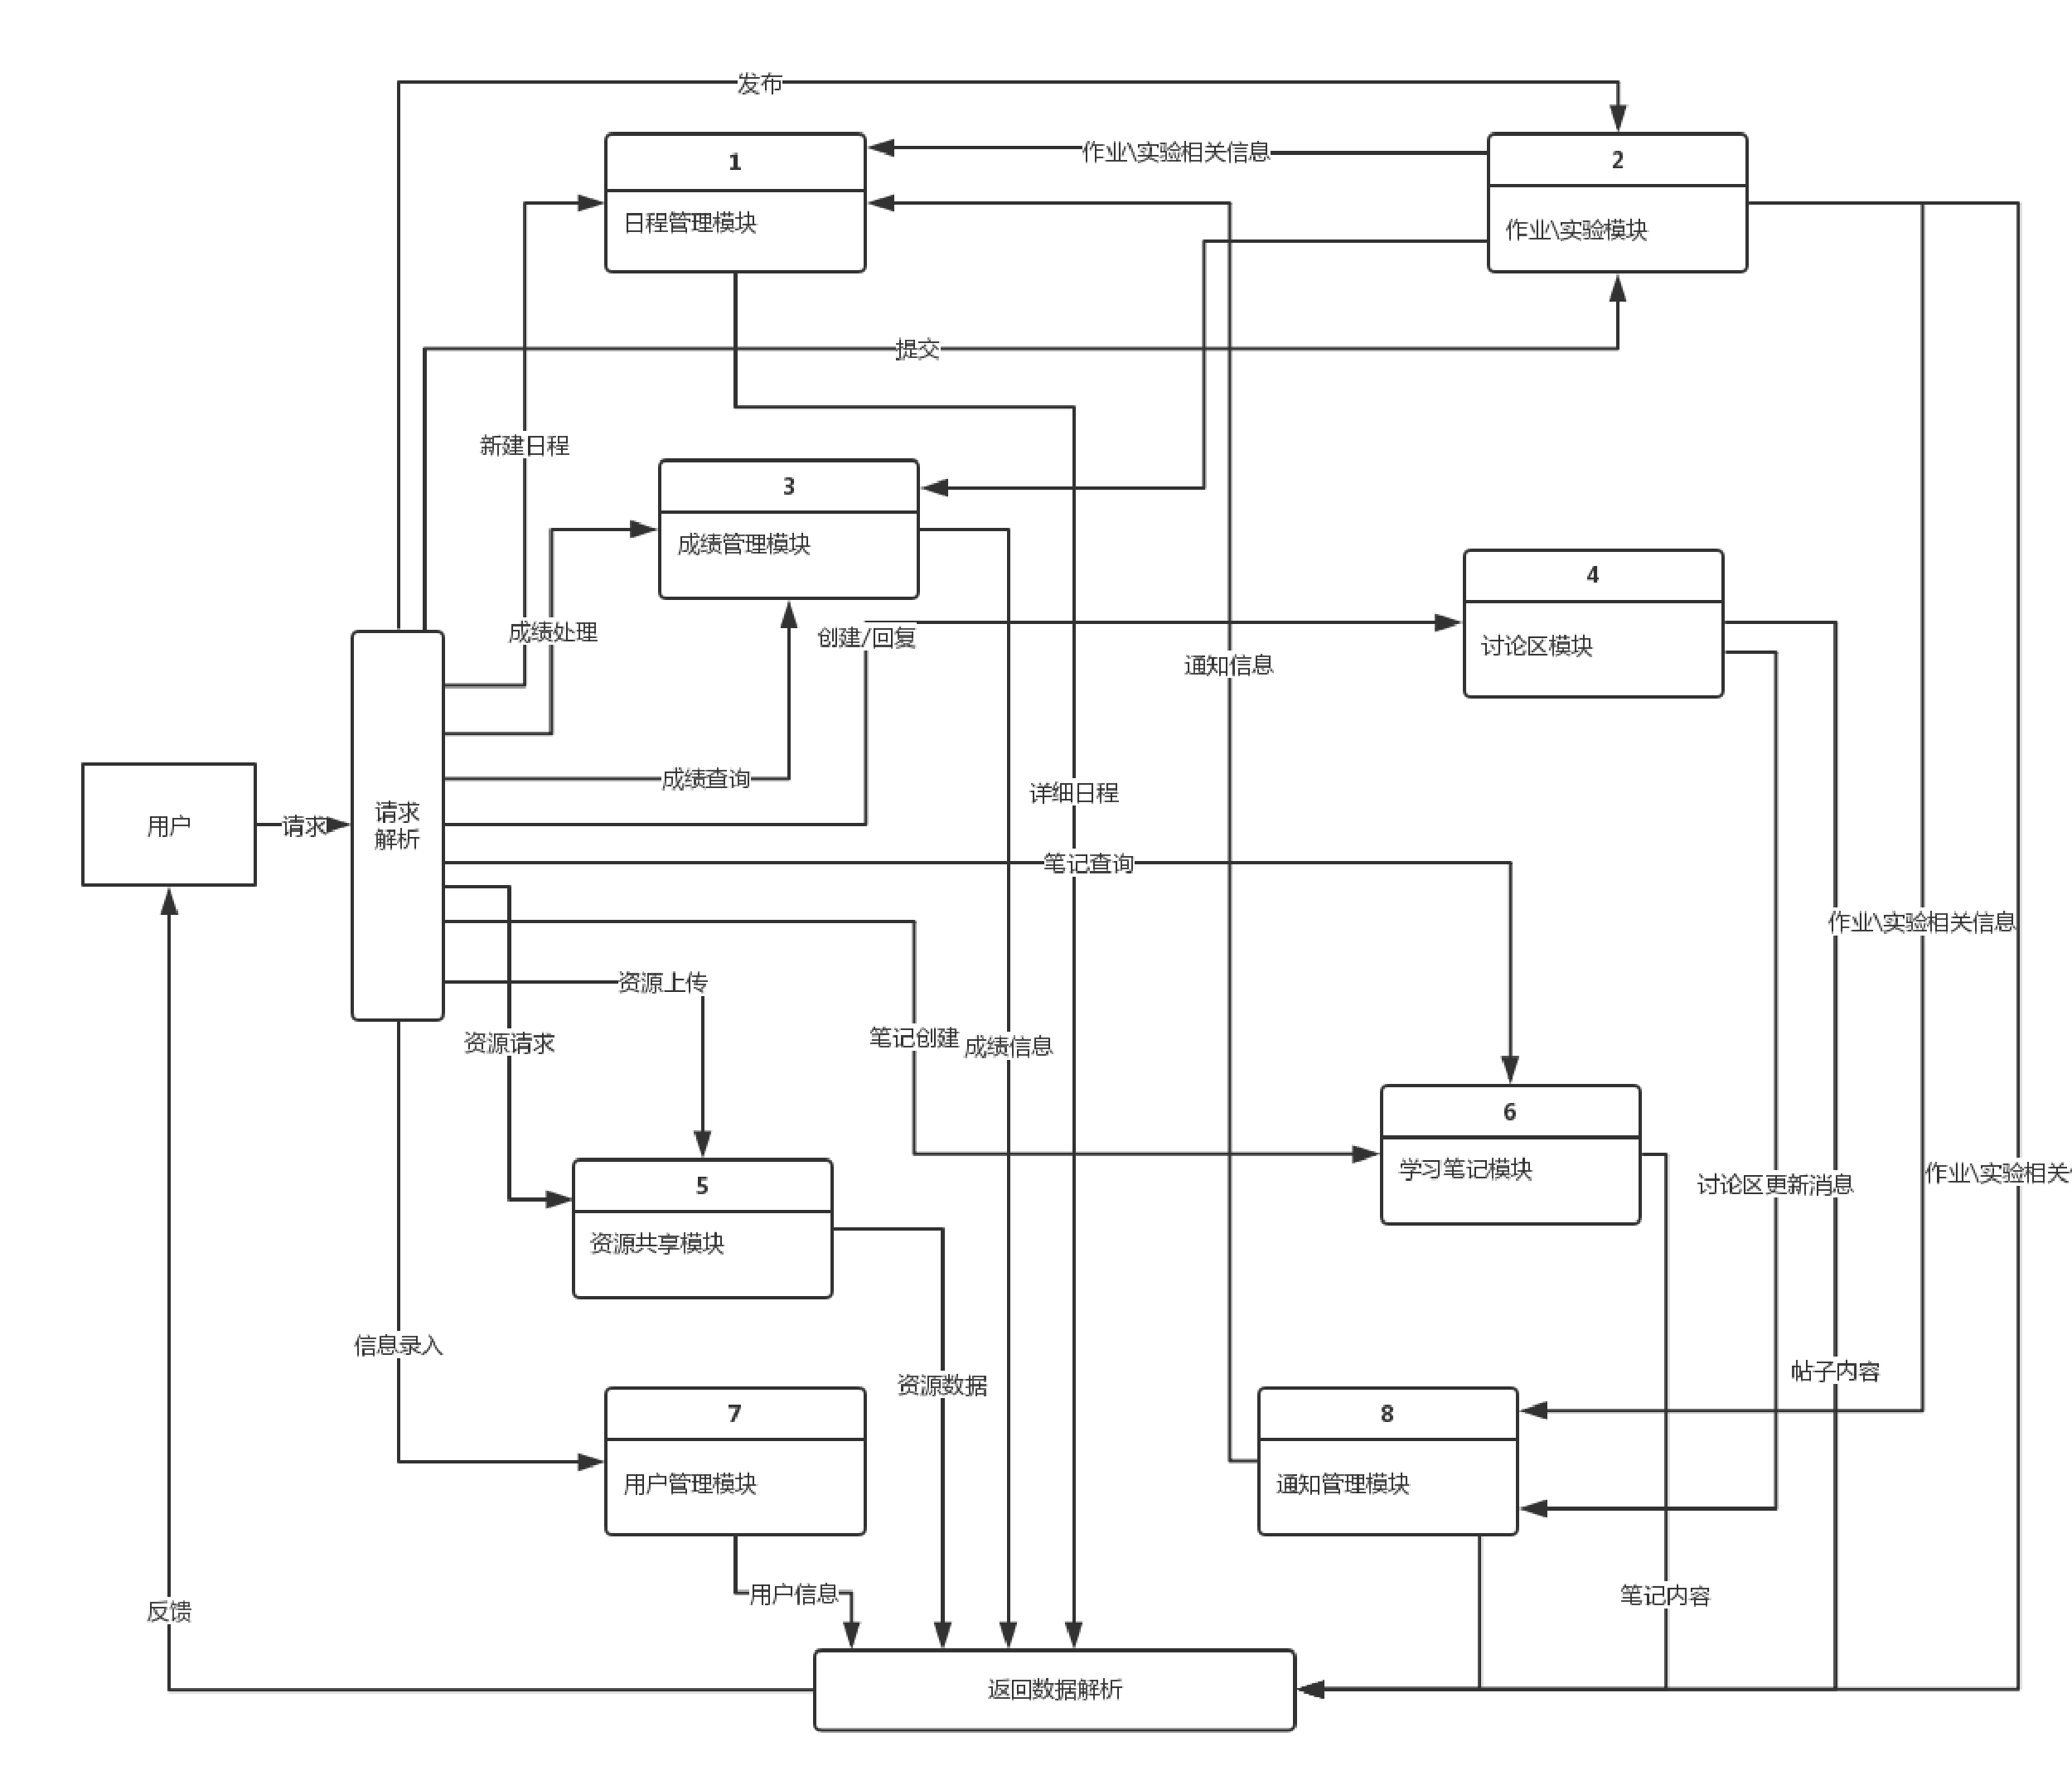
\includegraphics[width=15cm]{Level_0}
\caption{0层数据流图}
\end{figure}
\subsection{1层数据流图}
\subsubsection{日程管理模块}
\begin{figure}[H]
\centering
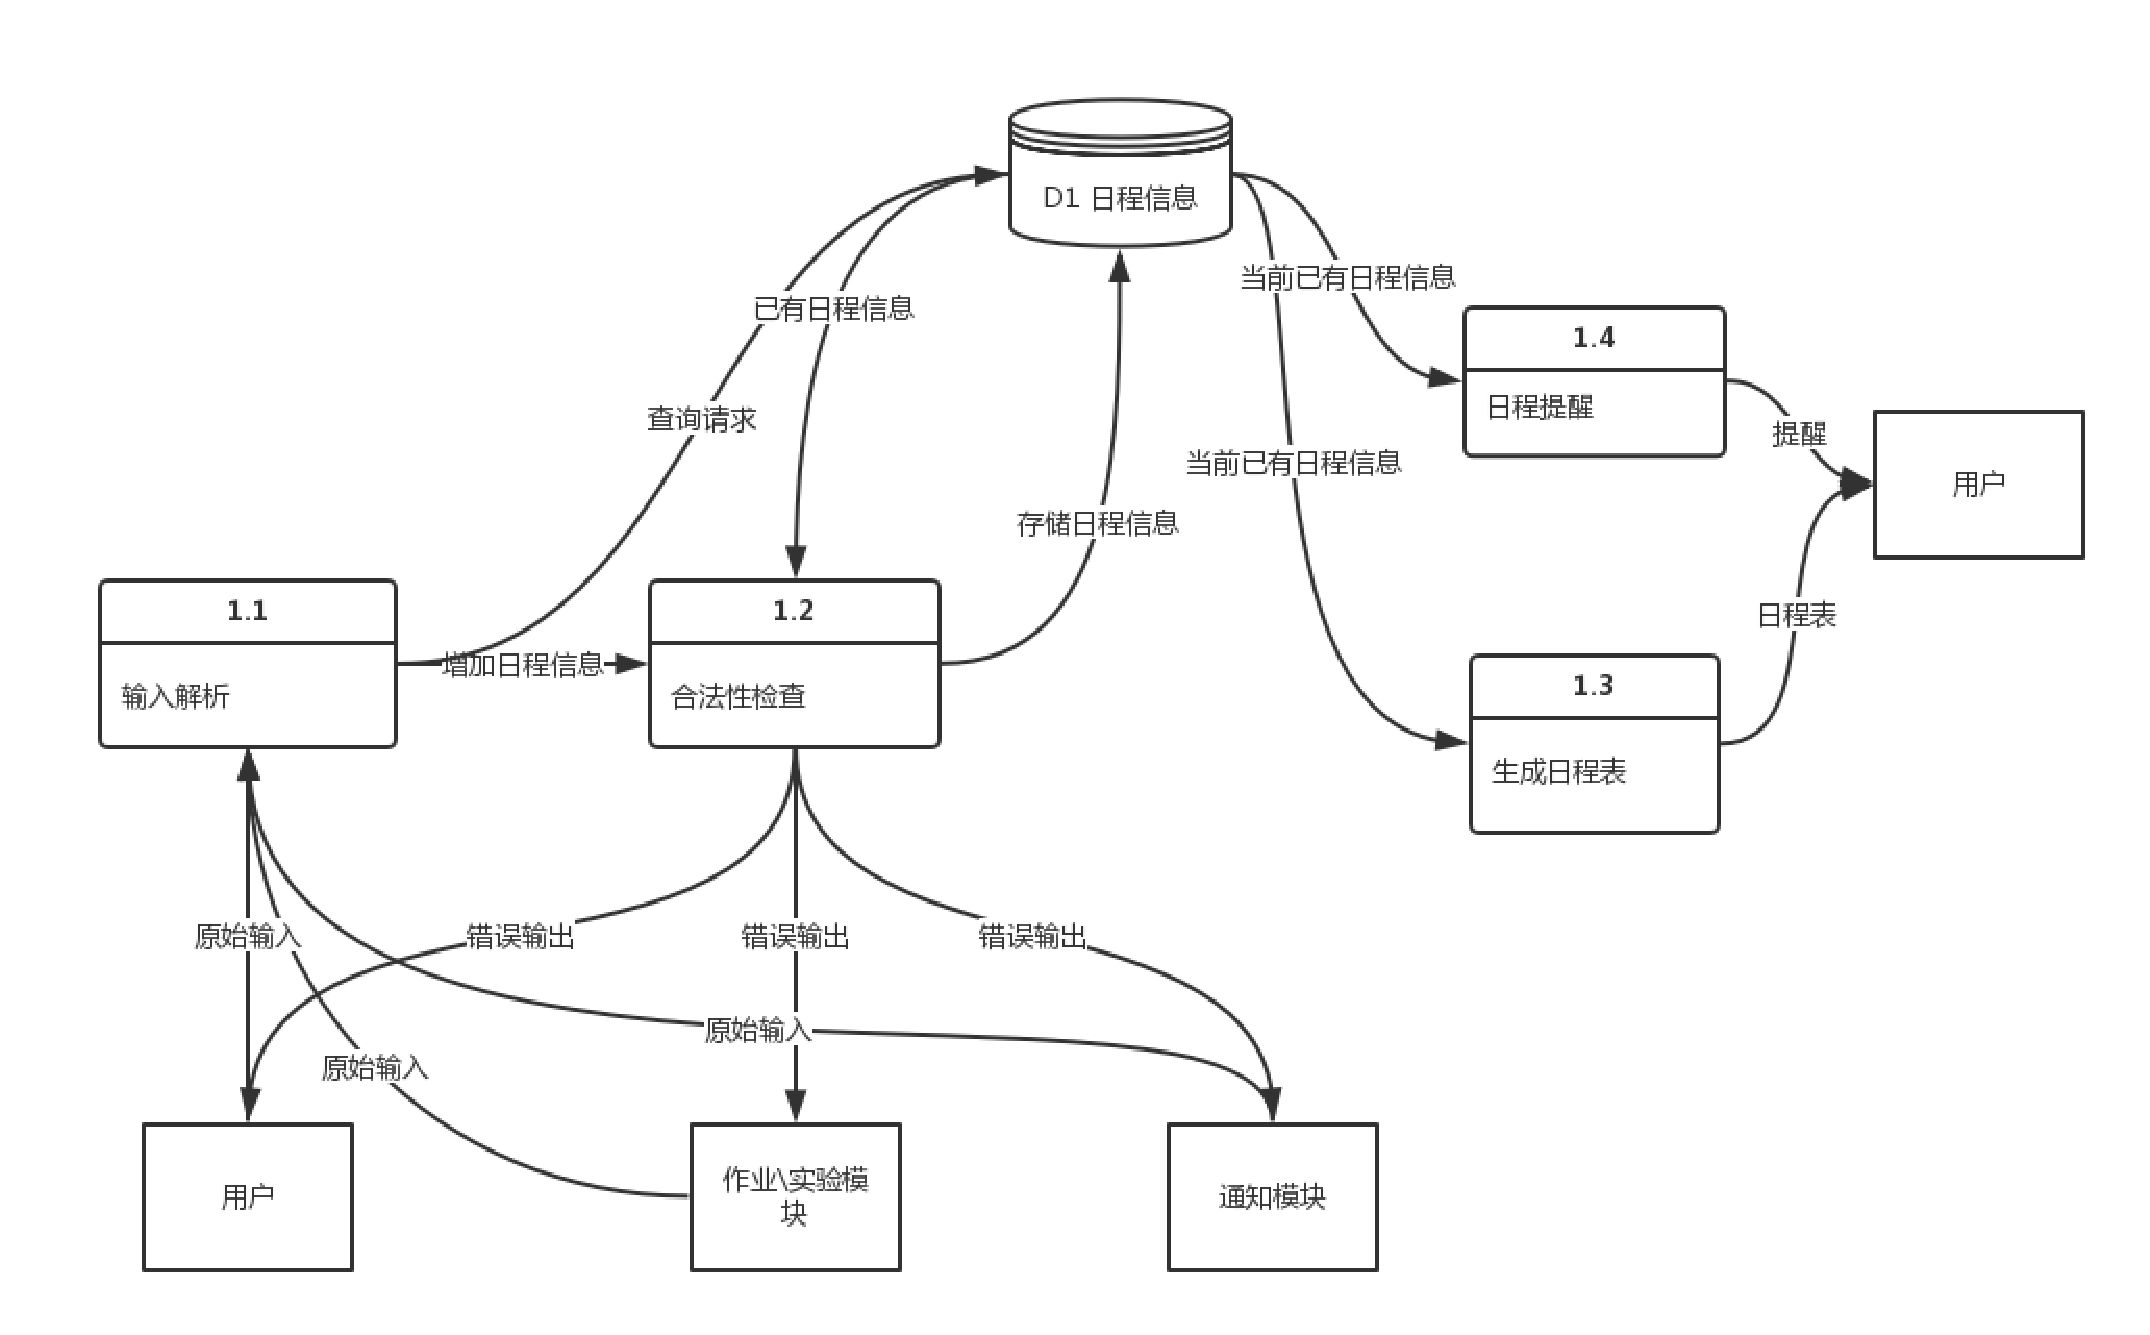
\includegraphics[width=15cm]{level1_1}
\caption{日程管理模块功能数据流图}
\end{figure}
\subsubsection{作业实验模块}
\begin{figure}[H]
\centering
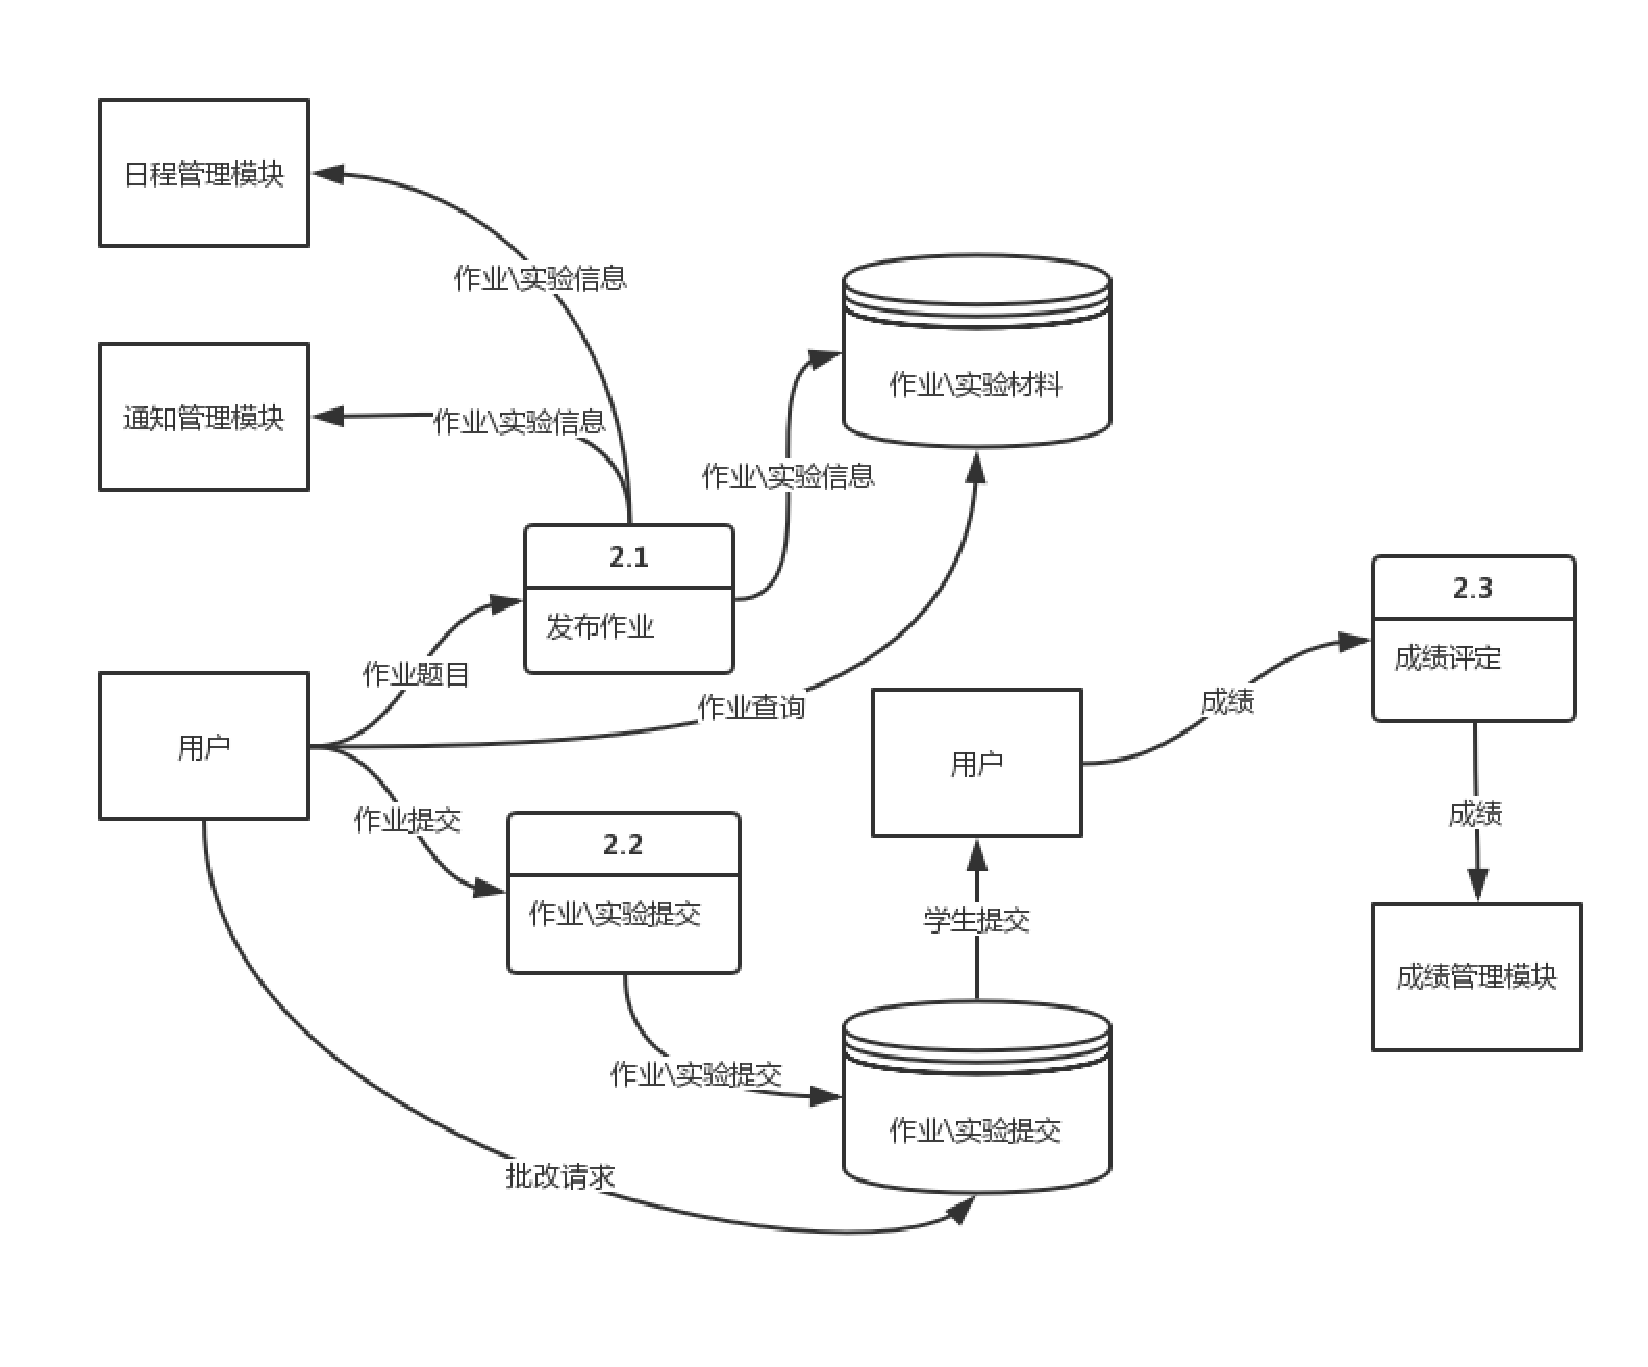
\includegraphics[width=15cm]{level1_2}
\caption{日程管理模块功能数据流图}
\end{figure}
\subsubsection{学习笔记模块}
\begin{figure}[H]
\centering
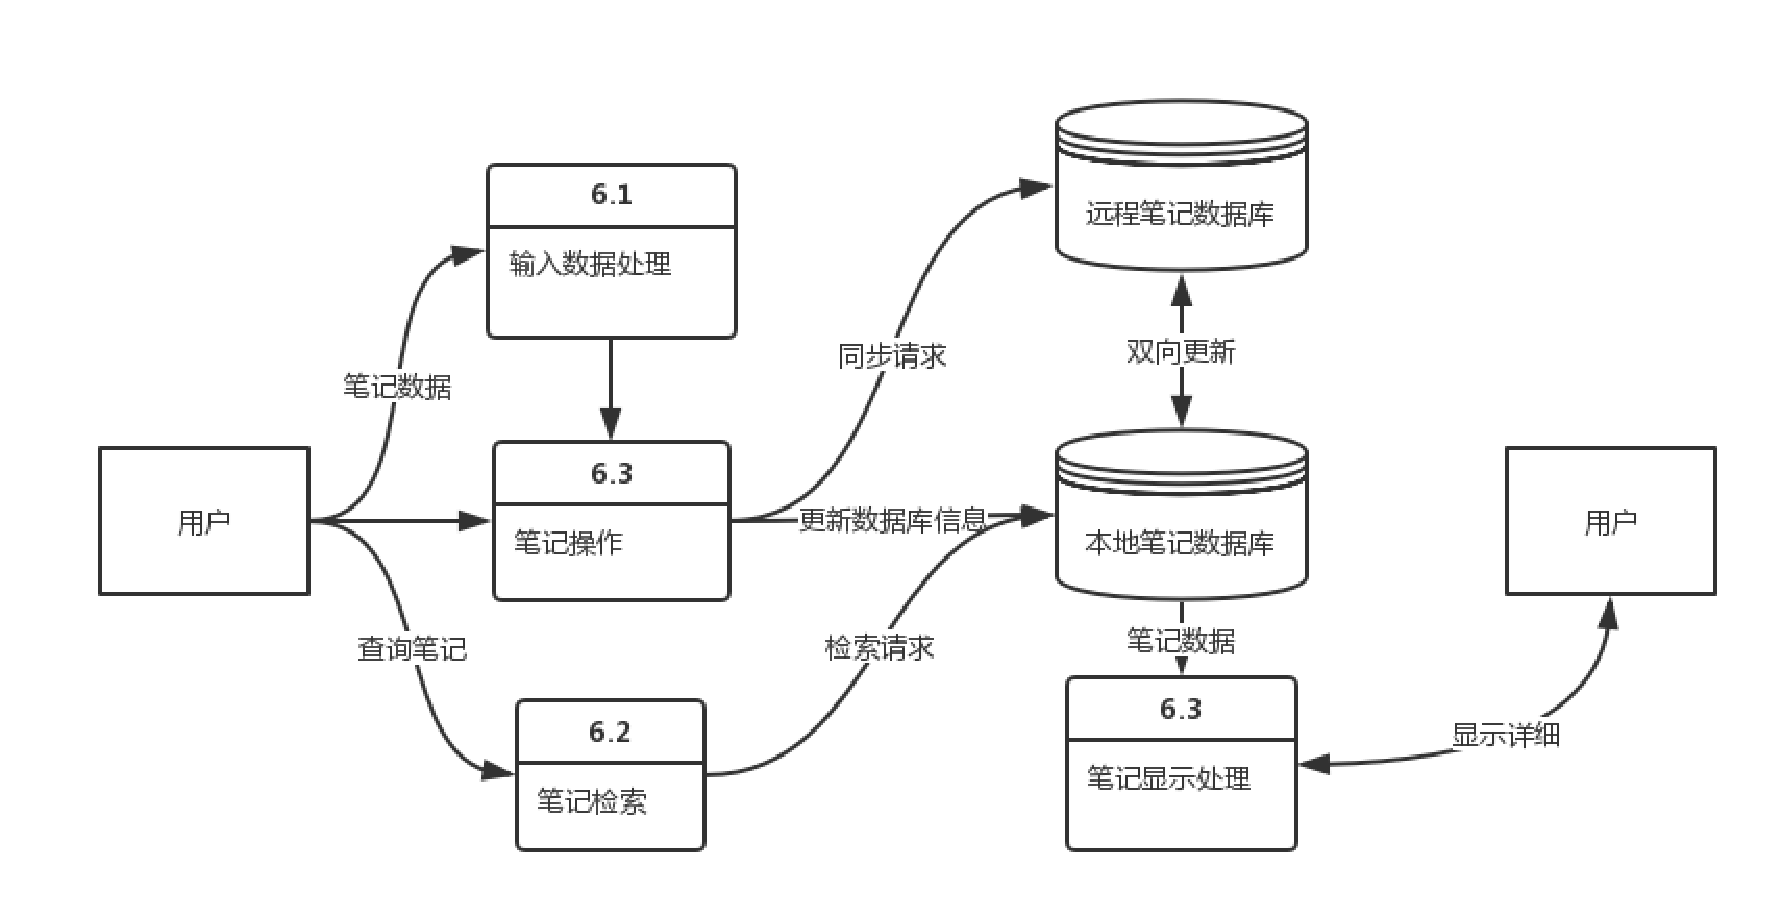
\includegraphics[width=15cm]{level1_3}
\caption{学习笔记模块功能数据流图}
\end{figure}
\subsubsection{成绩管理模块}
\begin{figure}[H]
\centering
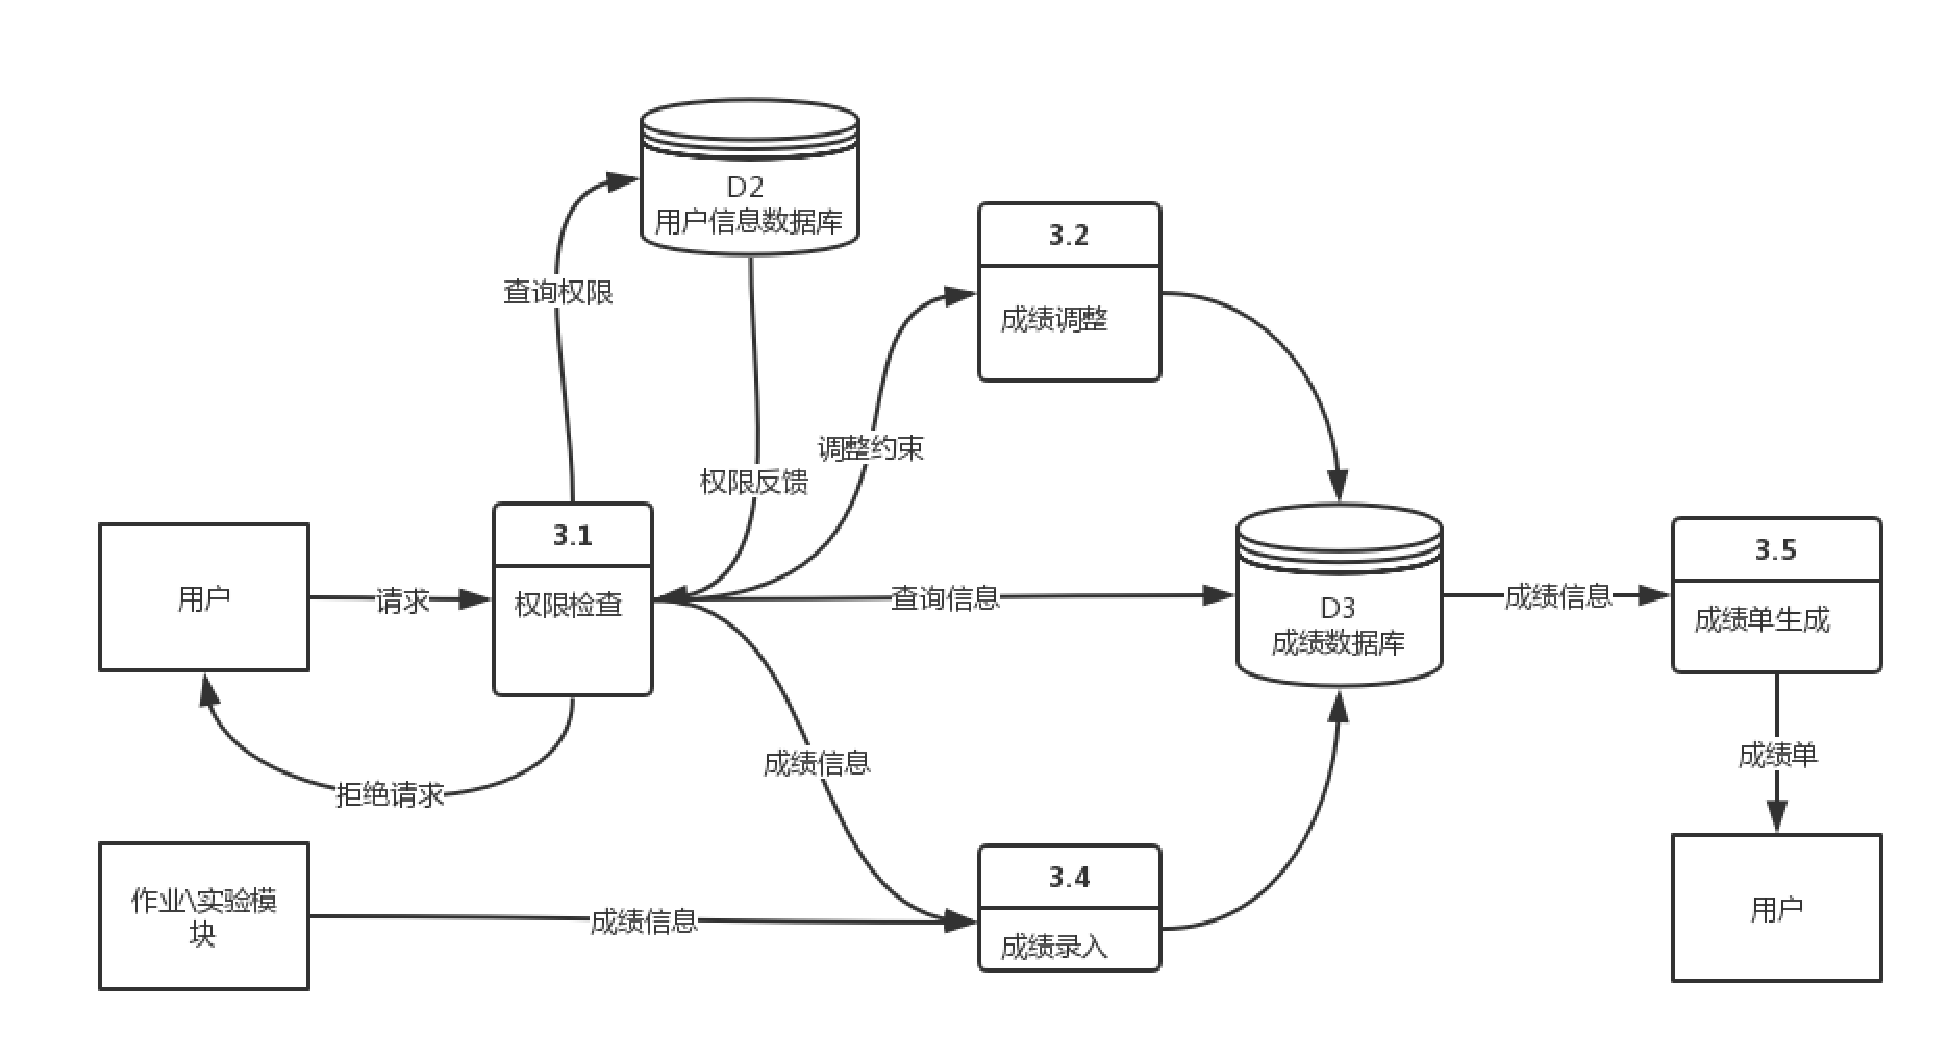
\includegraphics[width=15cm]{level1_4}
\caption{成绩管理模块功能数据流图}
\end{figure}
\subsubsection{用户管理模块}
\begin{figure}[H]
\centering
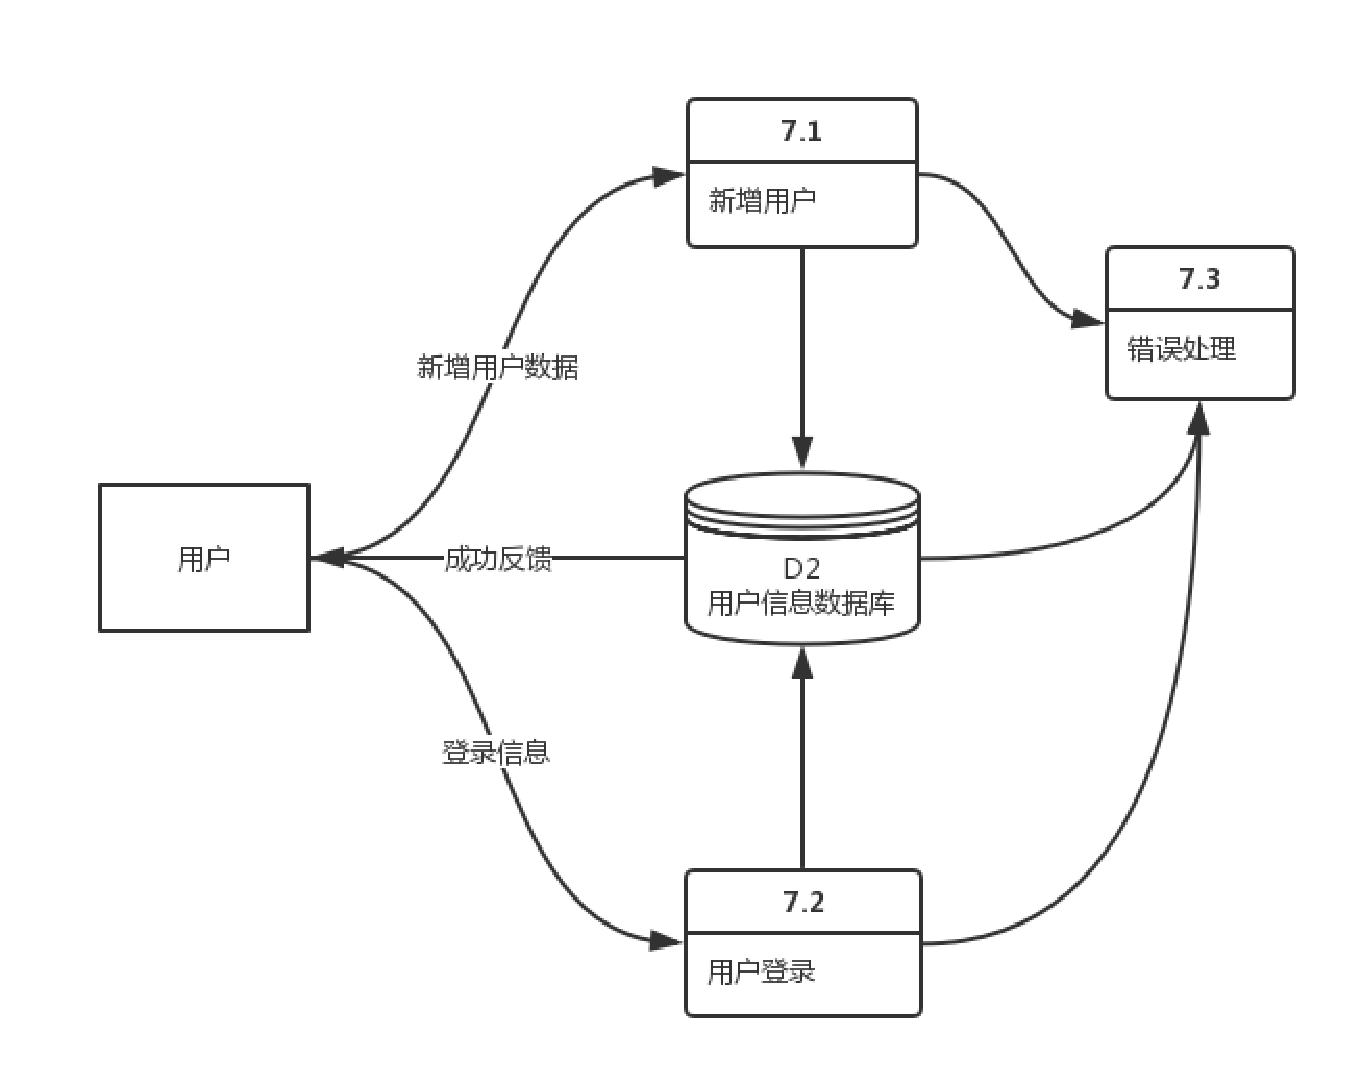
\includegraphics[width=15cm]{level1_5}
\caption{用户理模块功能数据流图}
\end{figure}
\subsubsection{讨论区模块}
\begin{figure}[H]
\centering
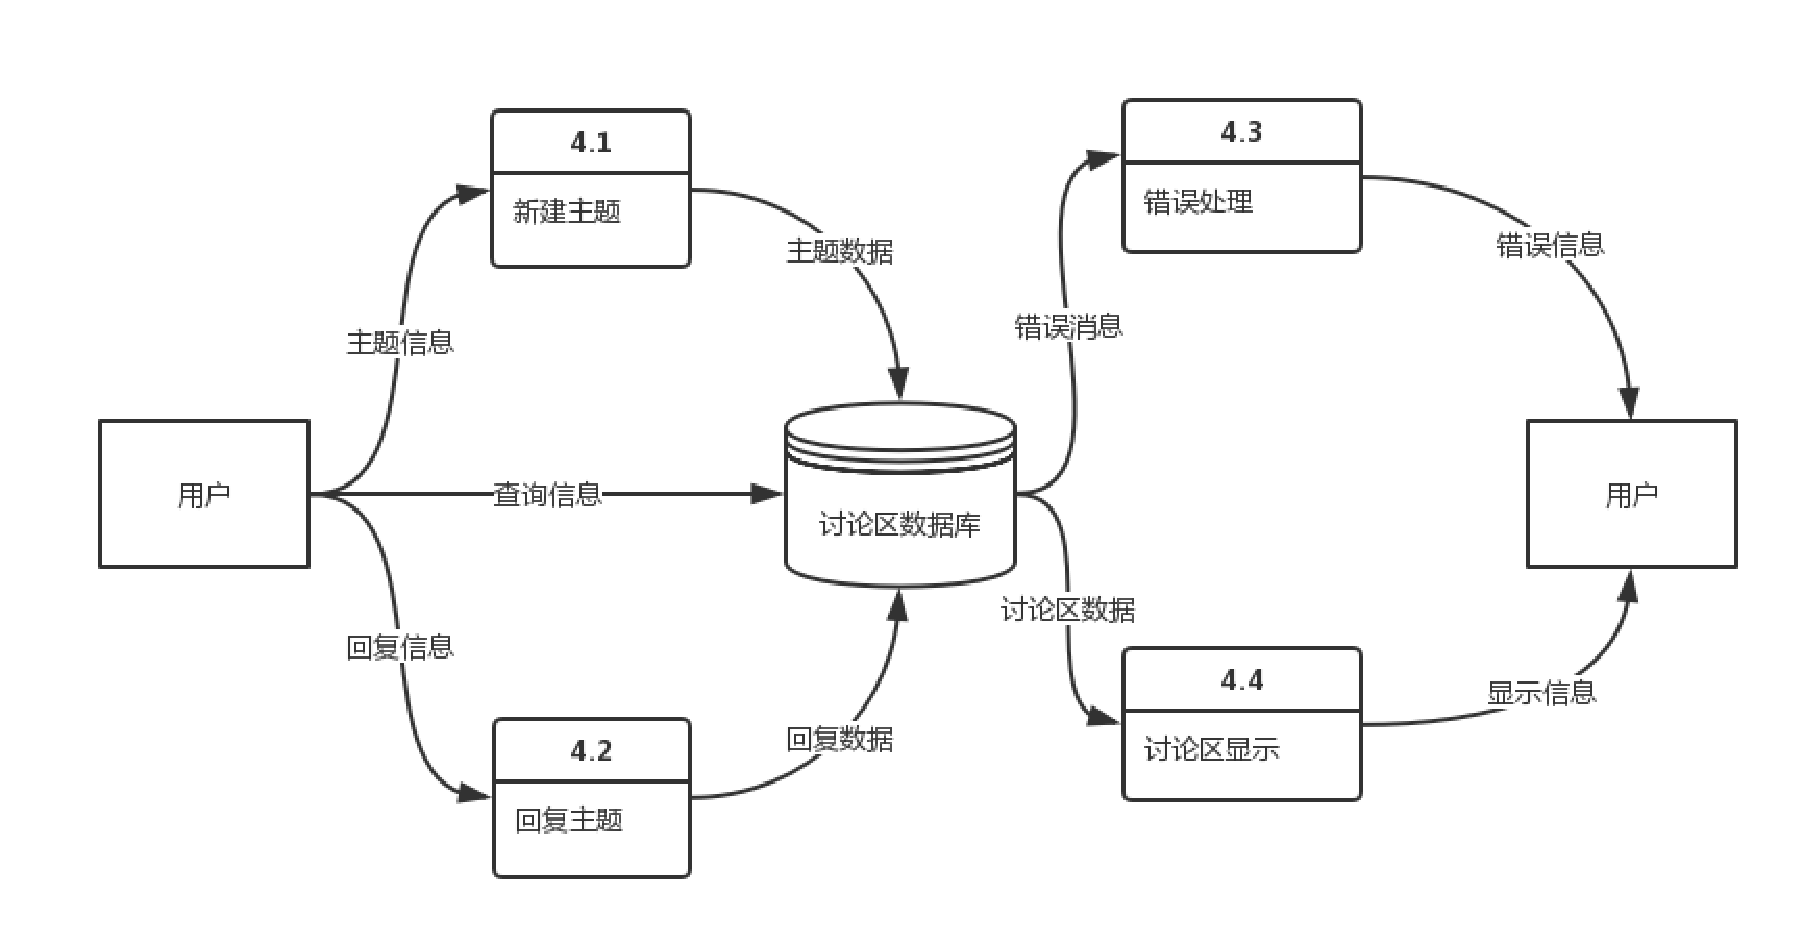
\includegraphics[width=15cm]{level1_6}
\caption{讨论区模块功能数据流图}
\end{figure}
\subsubsection{资源共享模块}
\begin{figure}[H]
\centering
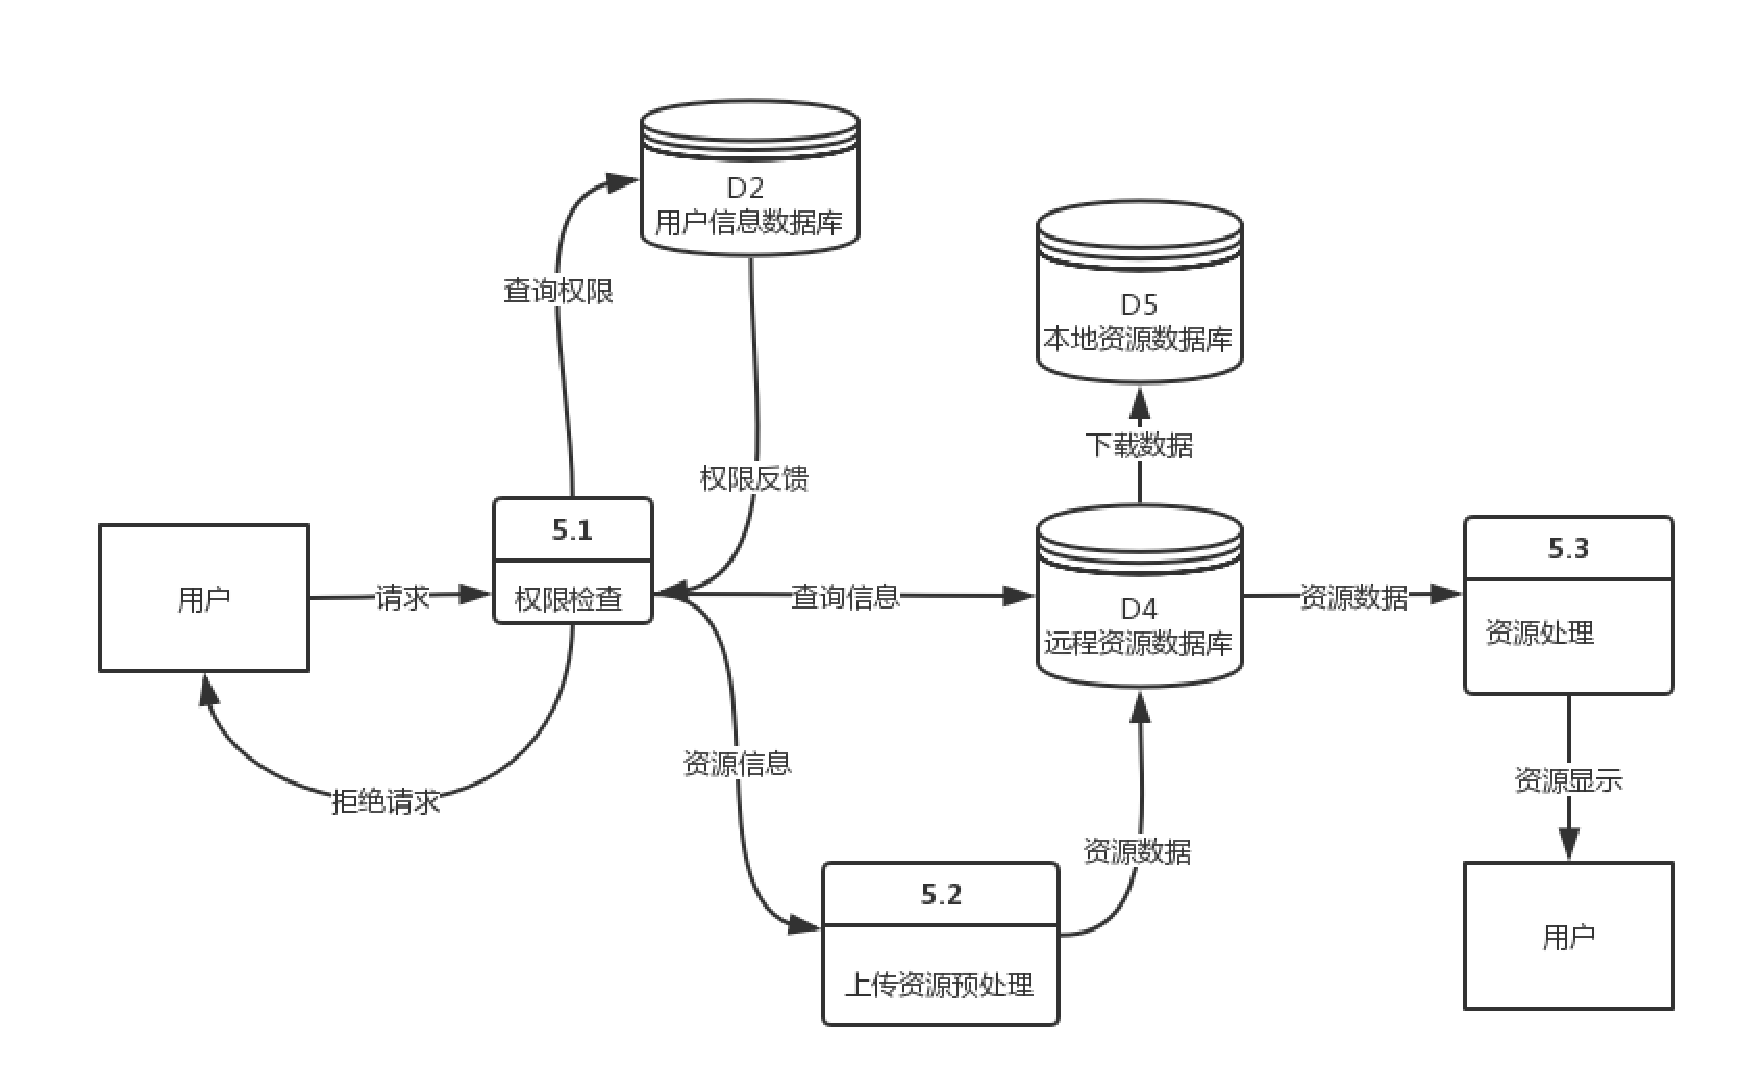
\includegraphics[width=15cm]{level1_7}
\caption{资源共享模块功能数据流图}
\end{figure}
\subsubsection{通知管理模块}
\begin{figure}[H]
\centering
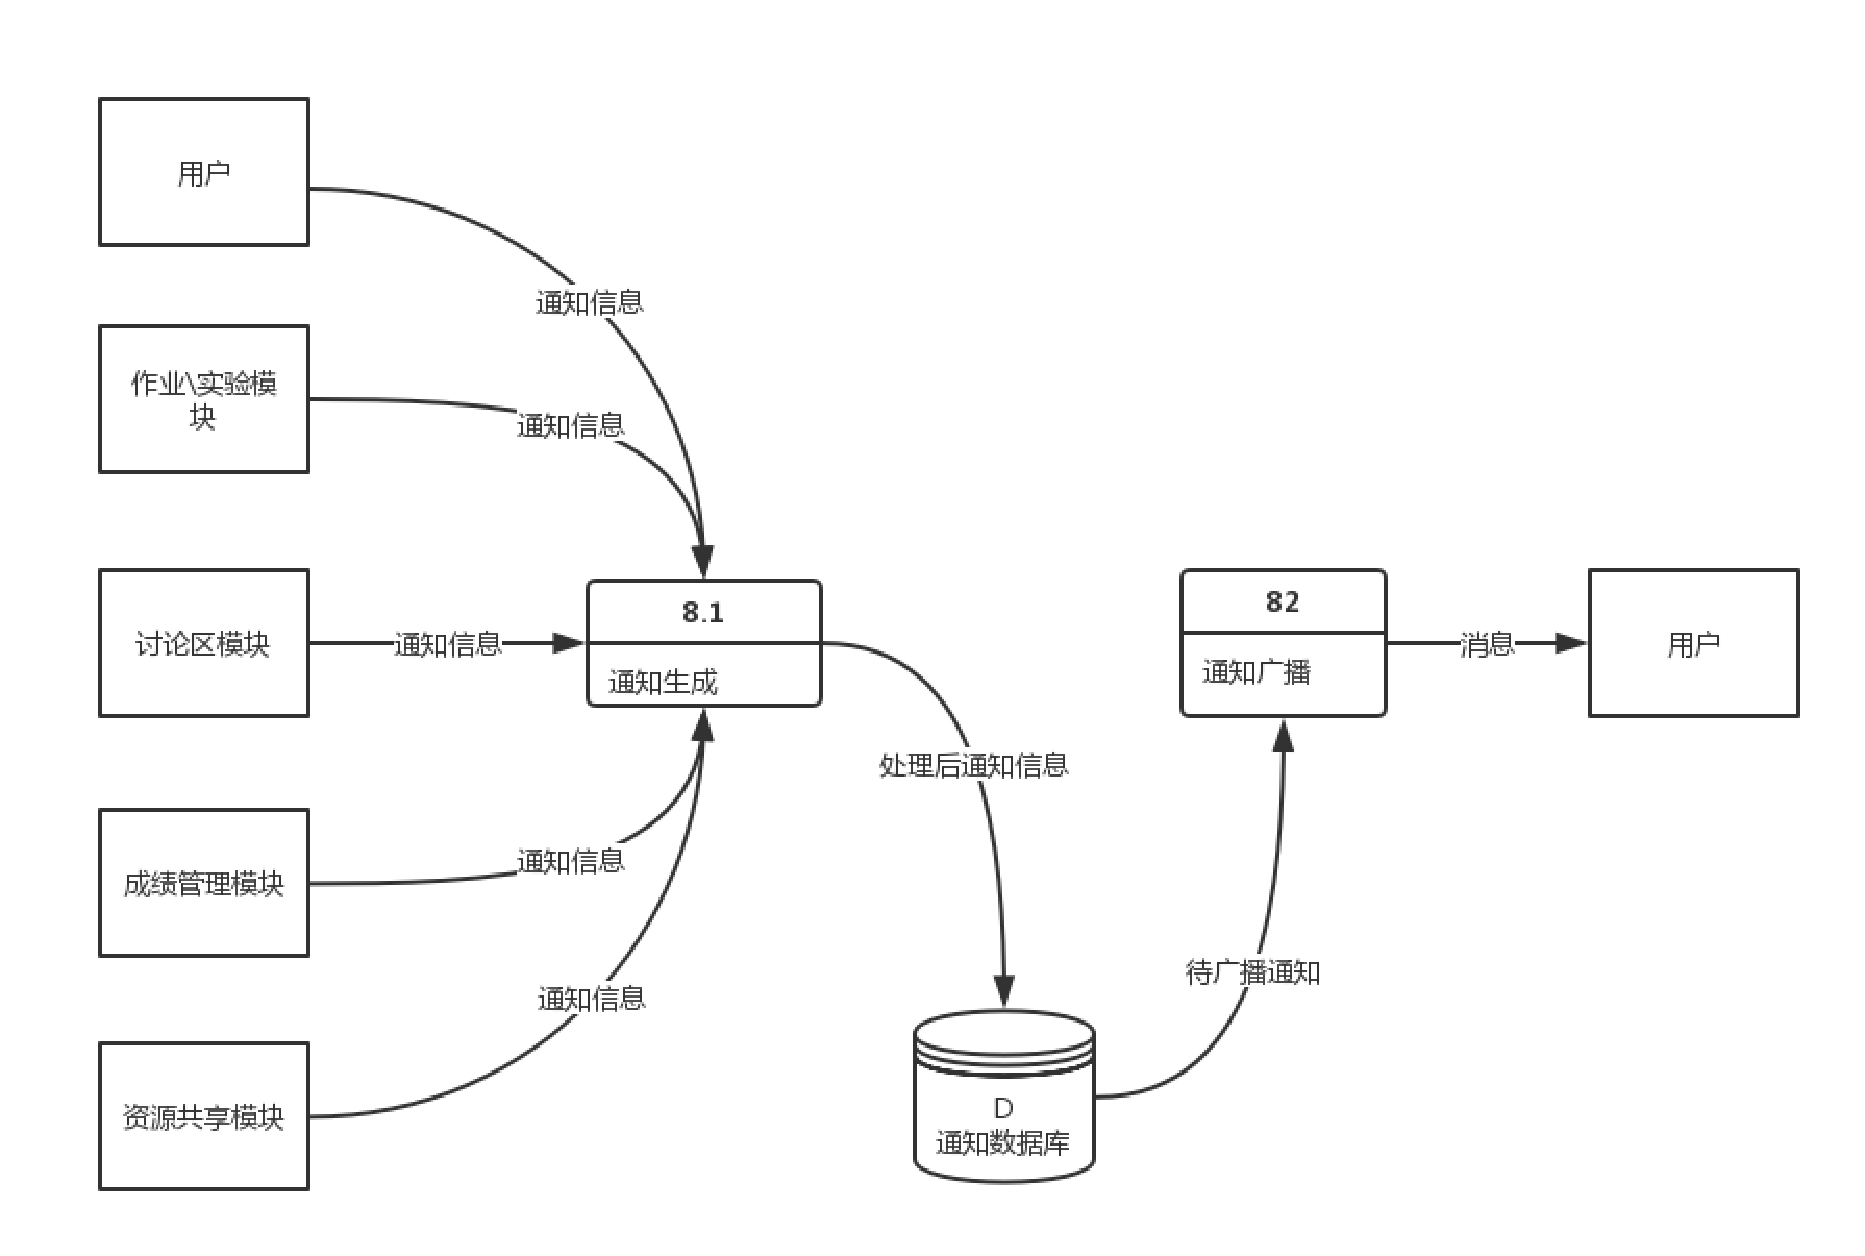
\includegraphics[width=15cm]{level1_8}
\caption{通知管理模块功能数据流图}
\end{figure}

\section{数据字典}
\subsection{数据流说明}
\subsubsection{请求}
\begin{description}
  \item[来源]用户
  \item[简述]用户对数据“请求操作”
  \item[去向]请求解析
\end{description}

\subsubsection{信息录入}
\begin{description}
  \item[来源]请求解析
  \item[简介]讲用户信息录入数据库
  \item[去向]用户管理模块
\end{description}

\subsubsection{用户信息}
\begin{description}
  \item[来源]用户管理模块
  \item[简介]从数据库中导出的用户信息
  \item[去向]返回数据解析
\end{description}

\subsubsection{反馈}
\begin{description}
  \item[来源]返回数据解析
  \item[简介]客户端对于用户数据的处理结果
  \item[去向]用户
\end{description}

\subsubsection{作业/实验/通知查询}
\begin{description}
  \item[来源]用户
  \item[简介]对作业/实验进行查询请求
  \item[去向]作业/实验材料,日程管理模块,通知模块
\end{description}

\subsubsection{作业/实验/通知发布}
\begin{description}
  \item[来源]用户
  \item[简介]新的作业/实验创建
  \item[去向]发布作业
\end{description}

\subsubsection{作业/实验/通知提交}
\begin{description}
  \item[来源]用户
  \item[简介]提交作业
  \item[去向]作业/实验提交
\end{description}

\subsubsection{作业/实验查看与批改}
\begin{description}
  \item[来源]请求解析
  \item[简介]查看学生提交的作业
  \item[去向]用户,本地数据库
\end{description}

\subsubsection{笔记创建}
\begin{description}
  \item[来源]请求解析
  \item[简介]新的笔记条目的创建
  \item[去向]学习笔记模块
\end{description}


\subsubsection{笔记内容}
\begin{description}
  \item[来源]学习笔记模块
\item[简介]用户查询的笔记内容
\item[去向]返回数据解析
\end{description}




\subsubsection{笔记数据}
\begin{description}
  \item[来源]用户,本地笔记数据库
\item[简介]用户的笔记内容
\item[去向]输入数据处理,笔记操作,笔记显示处理
\end{description}


\subsubsection{查询笔记}
\begin{description}
  \item[来源]用户
\item[简介]对笔记数据进行查询请求
\item[去向]笔记检索
\end{description}

\subsubsection{同步请求}
\begin{description}
  \item[来源]笔记操作
\item[简述]客户端与远程笔记同步
\item[去向]远程笔记数据库
\end{description}

\subsubsection{更新数据库信息}
\begin{description}
  \item[来源]笔记操作
\item[简述]向客户端提出更新数据库命令
\item[去向]本地笔记数据库
\end{description}


\subsubsection{双向更新}
\begin{description}
  \item[来源]远程笔记数据库,本地笔记数据库
\item[简述]客户端与远程笔记双向更新
\item[去向]远程笔记数据库,本地笔记数据库
\end{description}

\subsubsection{检索请求}
\begin{description}
  \item[来源]笔记检索
\item[简述]在客户端查询笔记
\item[去向]本地笔记数据库
\end{description}

\subsubsection{显示详细}
\begin{description}
  \item[来源]笔记显示处理
\item[简述]将笔记数据显示到用户界面
\item[去向]用户
\end{description}

\subsubsection{新增用户数据}
\begin{description}
  \item[来源]用户
\item[简介]在数据库中增加用户
\item[去向]新增用户
\end{description}

\subsubsection{成功反馈}
\begin{description}
  \item[来源]用户信息数据库
\item[简介]反馈给用户新增数据成功
\item[去向]用户
\end{description}

\subsubsection{登录信息}
\begin{description}
  \item[来源]用户,用户登录
\item[简介]将用户的登录信息在用户和客户端间同步
\item[去向]用户,用户登录
\end{description}

\subsubsection{主体信息}
\begin{description}
  \item[来源] 用户
  \item[简介] 新建主题以及简单描述
  \item[去向] 新建主题
\end{description}

\subsubsection{查询信息}
\begin{description}
  \item[来源] 用户
  \item[简介] 查询显示讨论区的相关信息
  \item[去向] 讨论区数据库
\end{description}

\subsubsection{回复信息}
\begin{description}
  \item[来源] 用户
  \item[简介] 回复内容
  \item[去向] 回复主题
\end{description}

\subsubsection{资源请求}
\begin{description}
  \item[来源] 用户
  \item[简介] 用户请求获取相关资源
  \item[去向] 权限检查
\end{description}

\subsubsection{查询权限}
\begin{description}
  \item[来源] 权限检查
  \item[简介] 检查用户的请求是否具有相应的执行权限
  \item[去向] 用户信息数据库
\end{description}




\subsection{数据存储说明}
\subsubsection{讨论区数据库}
\begin{description}
  \item[简述] 存储讨论区相关内容信息
  \item[数据排列] 降温被内容单独存储。同时以关键词等建立索引。并且另外建表存储创建者日期权限等信息
\end{description}

\subsubsection{本地资源数据库}
\begin{description}
  \item[简述] 存储用户下载和导入的本地资源数据
  \item[数据排列] 根据用户系统平台选用相应文件系统的存储方式。同时依据用户的选择建立权限等数据库表单
\end{description}
\subsubsection{远程资源数据库}
\begin{description}
  \item[简述] 存储用户服务器端的数据
  \item[数据排列] 分布式存储,尽量减少重复信息的存储。同时依据用户的选择建立权限等数据库表单
\end{description}
\subsubsection{日程信息数据库}
\begin{description}
  \item[简述] 存储用户日程相关信息
  \item[数据排列] 根据用户,日期,描述等键值建表
\end{description}
\subsubsection{成绩数据库}
\begin{description}
  \item[简述] 存储用户成绩相关信息
  \item[数据排列] 根据用户、成绩以及何次作业或者考试建表
\end{description}
\subsubsection{数据库发布作业/实验/通知存储}
\begin{description}
  \item[简述] 服务器数据库存放教师发布的作业/实验/通知
  \item[数据排列] 数据存在多个lable,主要的主键有发布课程编号,类型,作业号。其列名还有内容,截至日期,附件地址等。
\end{description}

\subsubsection{作业附件存储}
\begin{description}
  \item[简述] 服务器存放教师发布的作业/实验材料
  \item[数据排列] 不同的科目有不同的文件夹,存放到相应的文件夹下。将地址存入数据库相应的部分。
\end{description}

\subsubsection{学生提交作业/实验存储}
\begin{description}
  \item[简述] 服务器存放学生上传的作业/实验。
  \item[数据排列]数据库的主键为作业号。其列名还有学生学号,名称,作业/实验提交与否,地址。
  将学生提交的内容存入服务器的文件夹下,地址放入上述服务器。若使用git提交,则同样保存按照git服务器保存在服务器上。
\end{description}

\subsubsection{用户账号数据库存储}
\begin{description}
  \item[简述]服务器端数据库存储用户的邮箱,学号,姓名,密码,用户权限,选修课程,课程详情等基本信息
  \item[数据排列]数据存在多个table,以用户邮箱,学生姓名,课程名称为主键,数据按主键排列
\end{description}

\subsubsection{笔记数据库存储}
\begin{description}
\item[简述]存储在服务器数据库中的用户信息,笔记内容,笔记创建时间,相关学科等信息
\item[数据排列]数据存在多个table,数据以用户账户,笔记学科为主键,笔记按主键排列。
\end{description}

\subsubsection{笔记数据库本地存储}
\begin{description}
\item[简述] 存储在客户端数据库中的笔记内容,笔记创建时间,相关学科等信息
\item[数据排列] 数据存在多个table,数据以笔记创建时间,笔记学科为主键,笔记按主键排列。
\end{description}






\subsection{加工说明}
\subsubsection{新建主题}
检查用户提供信息是否合法。然后将其中的图片公式等等转换格式存入数据库中。
\subsubsection{回复信息}
检查用户回复是否合法。然后将其中的图片公式等等转换格式存入数据库中。
\subsubsection{讨论区显示}
从数据库中获取相关信息,处理渲染之后发送给用户客户端显示。
\subsubsection{权限检查}
根据用户请求从数据库中获取相关数据并判断是否具有执行操作的权限。
\subsubsection{上传资源预处理}
首先检查上传数据是否有效合法。不合法或者失效给出警告。合法则计算MD5查询数据库中是否已经存在相同资源,存在则只建立相应的链接,不存在则上传文件至远程数据库。
\subsubsection{资源处理}
从远程获取数据,根据数据格式以及用户平台进行相应的转码处理最后交付客户端直接进行显示。
\subsubsection{输入解析}
日程的输入有多种格式,如果用户输入的不是标准的各项信息,而是纯文本等等,则首先尝试从中解析出事件地点描述等关键信息,尝试构建日程,成功则存入数据库,失败返回报错。
\subsubsection{日程提醒}
检索当前日程数据库中的相关信息,比较当前日期,如果有满足提醒条件的则给用户发送提醒。
\subsubsection{成绩录入}
根据用户或者其他模块的输入构造满足后台数据存储结构的信息并且存储。
\subsubsection{成绩调整}
解析用户的调整需求看是否合法,如果合法则对数据库进行更新。

\subsubsection{发布作业/实验/通知}
用户将作业/实验/通知填写好发送。

服务器判断用户发来的数据,将附件存入相应空间,将其他内容存入数据库中。

向客户端发送成功与否的信息。

\subsubsection{学生提交作业/实验}
学生将作业/实验内容从本地提交。

服务器接受消息,更新数据库,并将收到的文件存储。

向客户端发送结果信息。

\subsubsection{处理登录}
客户端发送查询请求到服务器用户数据库,匹配该用户邮箱或学号和密码,匹配成功则返回成功登录的信息,并同步数据。匹配失败则返回失败信息,并显示账户不存在或密码错误。

\subsubsection{处理新用户请求}
客户端发送新建请求到服务器数据库,检查是否为新用户,若可创建则返回允许创建信息,失败则返回无法创建新用户。

\subsubsection{处理笔记}
对笔记请求数据处理,分发给下一级功能区具体处理

\subsubsection{创建笔记}
创建新的笔记,创建成功则将新的笔记按用户选择存入本地存储,或存入服务器。

\subsubsection{删除笔记}
删除云端或者本地存储的笔记,返回操作结果。

\subsubsection{处理查询}
从本地存储和服务器存储的的数据文件进行搜索,对于符合关键字的搜索返回给用户,如果没有结果则显示无结果。



\end{document}
